\documentclass[a4paper,12pt]{report} % Format du papier, type de document
 
\usepackage[utf8]{inputenc} % Permet de tapper les accents tels quels
\usepackage[T1]{fontenc} % Permet l'utilisation d'accents
\usepackage[french]{babel} % Dit que le document est en français
\usepackage{amsfonts} % Différents packages... Lire la doc....
\usepackage{amsmath}
\usepackage{listings}
\usepackage{color}
\usepackage{graphicx} %affichage d'image
\usepackage{moreverb}
\usepackage[colorlinks=true,linkcolor=black]{hyperref} %lien hypertexte
\usepackage{fullpage}
\usepackage{fancyhdr}
\pagestyle{fancy}
\renewcommand{\thesection}{\arabic{section}}
\setcounter{tocdepth}{5}
\setcounter{secnumdepth}{5}

\renewcommand{\headrulewidth}{0pt} 
\fancyhead{} %retire en tete

\renewcommand{\footrulewidth}{1pt} %bas de page
\fancyfoot[C]{\textbf{\thepage}} 
\fancyfoot[L]{Software evolution}
\fancyfoot[R]{Jpacman framework}

\title{Software evolution \\ JPacman framework}
\author{Ducruet Corentin \\ Gallois Florent \\ Ledru Santorin}
\date{Année académique\\2015 - 2016}
%\begin{figure}[!h] %on ouvre l'environnement figure
%		\centering
%		\includegraphics[width=108mm,height=65mm]{impulsion.png}
%	\end{figure} 

%\begin{figure}%[H] si on veut que l image soit a cet endroit
%	\centering
%	\includegraphics[width=108mm,height=65mm]{./scr/logo}
%	\caption{Icône}
%	\label{fig:Icône}
%\end{figure}

\begin{document} 
\maketitle
\newpage 
\addtocontents{toc}{\protect\thispagestyle{fancy}} %modifie mise en page table des matiere
\tableofcontents
\newpage
%\raggedright
\section{Introduction}
Dans le cadre du cours de Softare Evolution, l'occasion nous est donnée de mettre en pratique les concepts d'évolution logicielle vus en cours. Le projet qui nous est confié consiste à récupérer un projet de Pac-Man et d'y implémenter plusieurs fonctionnalités. Ces mêmes fonctionnalités doivent être réalisées en suivant un processus de développement dirigé par les tests. Après la réalisation de ces tâches, il nous est demandé de rassembler ces différents travaux dans le logiciel. Enfin, une analyse de la qualité ainsi qu'une amélioration du code doit nous permettre de terminer le logiciel.

Dans un premier temps, nous étudions chaque tâche individuelle par la réalisation de la "Supergomme", ensuite, la série de labyrinthe et enfin, l'implémentation de l'IA des fantômes.

Dans un deuxième temps, nous exposons les difficultés rencontrées lors de la fusion des trois fonctionnalités. En dernier lieu, l'analyse du code et des améliorations sont abordées.

Ce rapport s'achève par une brève conclusion.

\section{Supergomme - Ducruet Corentin}
\subsection{Programme initial et objectifs}
La version initiale du framework Jpacman ne contenait qu'un seul type de gomme qui avait pour effet d'augmenter notre score de 10 points. Il nous a été demandé d'ajouter la fonctionnalité "Supergomme". Cette fonctionnalité ajoute un nouveau type de gomme : les "Supergommes". Celles-ci se distinguent des autres gommes par la variation de leurs effets.

Tout d'abord, elles sont rouges afin de les différencier visuellement. Ensuite, lorsqu'elles sont mangées par Pac-Man, le score est augmenté de 50 points et les rôles sont inversés : en effet, Pac-Man devient chasseur et les fantômes deviennent les proies pendant 7 secondes lors des deux premières "Supergommes" mangées et durant 5 secondes pour les deux dernières. Lorsque les fantômes sont les proies, ils sont bleus et fuient Pac-Man. Dans le cas où Pac-Man arrive à manger un fantôme, cela lui rapporte des points : 200 pour le premier, 400 pour le deuxième, 800 pour le troisième et 1600 pour le quatrième.

\subsection{Démarche suivie}
Pour réaliser cette fonctionnalité, nous avons tout d'abord créer une classe "SuperPellet" qui hérite de "Pellet". Nous l'avons ajoutée à la "MapParser" pour que les "Supergommes" soient également présentes sur la carte.

Nous avons créé une classe "VulnerableGhost" qui représente les fantômes pouvant être chassés quand une "Supergomme" est mangée. Les fantômes prénommés Blinky, Clyde, Inky et Pinky héritent donc dorénavant de "VulnerableGhost". Dans le même temps, une classe "VulnerableGhostFactory" a été réalisée. Cette dernière hérite de la classe "GhostFactory" qui sert à instancier les fantômes et permet de respecter le Factory Design Pattern.

Pour gérer l'alternance des modes, nous avons développé un timer qu'il est possible de mettre en pause. De cette manière, lorsque le jeu est en mode pause, le timer ne continue pas de s'exécuter.

Les collisions sont gérées dans "PlayerCollisionSuperPellet". Si Pac-Man mange une "Supergomme", le mode "chasseur" est déclenché: les fantômes deviennent bleu et fuient Pac-Man. Pendant ce temps, un timer est lancé pour qu'après 7 secondes (pour les deux premières "Supergommes", 5 secondes pour les deux dernières) le jeu reprenne son cours habituel. Dans le cas où, Pac-Man mange un fantôme durant le mode "chasseur", il gagne le score prédéterminé (voir Programme initial et objectifs).

Enfin, nous avons créé un launcher nommé "LauncherSuperPellet" afin de démarrer le jeu accompagné des paramètres permettant que les "Supergommes" soient activées.

\section{Série de labyrinthe - Ledru Santorin}
\subsection{Programme initial et objectifs}
A l'origine, Pac-Man mourrait et la partie s'achevait à partir du moment où un fantôme
rentrait en contact avec lui. La partie prenait fin également lorsque
le joueur avait ramassé toutes les gommes du labyrinthe de base proposé.

Il nous a été demandé de mettre en place la fonctionnalité "Série de labyrinthe". Elle se caractérise par plusieurs objectifs.

Le premier objectif vise à donner à Pac-Man trois vies. Lorsqu'il
meurt, il est téléporté sur une case aléatoire située à plus de quatre cases
du fantôme le plus proche. Pac-Man doit également gagner une vie tous
les dix milles points accumulés.

Ensuite, un système de niveaux a été réalisé. Lorsqu'un
niveau est terminé, la partie s'enchaîne sur le niveau suivant. Pac-Man
conserve son nombre de vies et ses points lors du changement de niveau.

Enfin, la progression du joueur doit pouvoir être sauvegardée pour
qu'il puisse reprendre sa partie au dernier niveau atteint.

\subsection{Démarche suivie}
\subsubsection{Still alive!}
Tout d'abord, une simple variable est ajoutée dans la classe "Player"
dans le but de tenir le compte des vies restantes de Pac-Man. Le décompte des
vies se fait grâce à la méthode "setAlive(boolean)" de la classe "Player".
La résurrection de Pac-Man est effectuée dans la méthode "levelLost()" de
la classe "SinglePlayerGame", un Observer étant déjà en place, nous nous en sommes servi. Dans cette méthode, lorsque le joueur possède encore une vie,
une case aléatoire du plateau de jeu est choisie à partir de la méthode "nearestValidRespawnPoint()". On déplace Pac-Man sur la position de résurrection valide la plus proche.

\subsubsection{Plusieurs niveaux}
On gère d'abord le chargement de plusieurs niveaux. Les niveaux chargés
se réfèrent à tous les fichiers nommés "board{*}.txt" présents dans le dossier
"ressources" des fichiers du jeu. Ils sont toujours présentés au joueur
dans l'ordre alphabétique des noms des fichiers. Ils sont chargés dans
un tableau de "Levels". "SinglePlayerGame" a été modifié pour qu'il puisse
gérer plusieurs niveaux. Dorénavant, il existe deux moyens de changer de niveau :
 d'une part, des boutons ont été implémentés afin de choisir son niveau dès le début de la partie; d'autre part, l'unique autre manière de changer de niveau est de gagné le niveau en cours de partie. A ce moment,
le changement de niveau se fait toujours grâce à l'"Observer" présent
dans la classe "SinglePlayerGame", mais cette fois dans la méthode "levelWon()".


\subsubsection{Sauvegarde de progression}
En début de partie, le programme demande le nom de l'utilisateur.
Le logiciel permet de vérifier s'il existe déjà un fichier de sauvegarde associé
à l'utilisateur, sinon celui-ci est créé. A chaque niveau est associé un
indice. Le plus grand indice des niveaux terminés par
le joueur est stocké dans le fichier de sauvegarde. Lors de la prochaine partie, si
l'utilisateur entre le même nom, il pourra choisir le niveau qu'il désire dans le cas où il l'a déja débloqué grâce aux boutons de changement
de niveaux de l'interface.


Un Observer Design Pattern a été implémenté par le biais de l'interface
"GameObserver" afin de permettre de notifier le joueur par des pop-up. Ces notifications ont lieu lorsque certains événements surviennent, tels que le fait de ne pas pouvoir démarrer un niveau (car le joueur ne l'a pas débloqué), quand le joueur a terminé sa partie et que la progression est sauvegardée.


\section{IA pour fantômes - Gallois Florent}
\subsection{Programme initial et objectifs}
Actuellement, les comportements des quatres fantômes du jeu Pac-Man sont erratiques : 
leur trajectoire est déterminée aléatoirement.

Nous avons créé des IA pour les fantômes afin de leur donner des trajets plus intéressants pour le jeu.
Pour cela, l'objectif est d'affecter à chaque fantôme deux modes : un mode de poursuite pendant lequel ils suivent une stratégie de poursuite et un mode de dispersion durant lequel ils suivent une trajectoire prédéfinie.

Le mode poursuite ayant déjà été réalisé dans le logiciel, nous avons réalisé le mode dispersion.
Pour ce faire, chaque fantôme doit régulièrement se rendre dans un coin : Pinky en haut à gauche, Blinky en haut à droite, Clyde en bas à gauche et enfin, Inky en bas à droite.

Nous avons implémenté ce mode par la réalisation d'un Strategy Design Pattern.
Ce changement de stratégie permet d'alterner entre la poursuite et la dispersion.
Ces variations se font selon les périodes de temps indiquées dans l'énoncé de base du projet : 7 secondes de dispersion, ensuite 20 secondes de poursuite, 7 secondes de dispersion,etc. 

\subsection{Démarche suivie}
La principale difficulté de cette réalisation est d'arriver à construire élégamment les IA des fantômes de telle sorte qu'un ajout de stratégie reste accessible.
Comme il nous l'a été suggéré, nous nous sommes intéréssés au Strategy Design Pattern.

\begin{figure}[!h] %on ouvre l'environnement figure
		\centering
		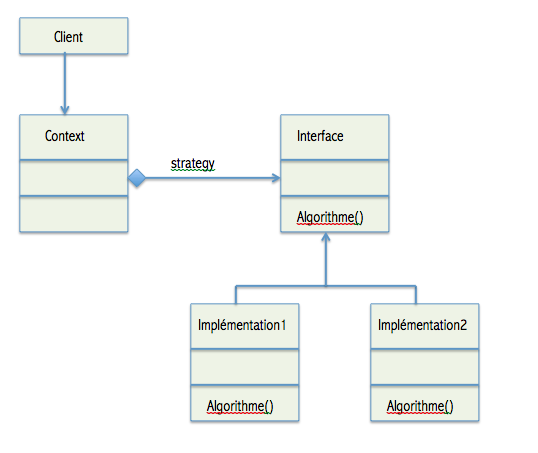
\includegraphics[scale=0.7]{ressources/StrategyDesignPattern.png}
		\caption{Strategy Design Pattern}
\end{figure} 



Ce pattern est très utile lorsqu'il est nécessaire de permuter dynamiquement des algorithmes ou, par exemple, lorsque des classes ne diffèrent que par leur comportement. Ainsi, pour éviter de dupliquer le code, une seule classe est créée. Celle-ci comprend alors les éléments de base ainsi qu'une interface implémentée par diverses classes décrivant les différents comportements de la classe centrale.

De prime abord, nous avions pensé créer pour chacun des fantômes, une interface implémentée par deux classes : une classe poursuite et une classe de dispersion.
Or cela engendrait toujours un code dupliqué, les algorithmes de dispersion étant tous les mêmes.

Pour la première version du logiciel, un pattern comme celui qui suit a été crée :

\begin{figure}[!h] %on ouvre l'environnement figure
		\centering
		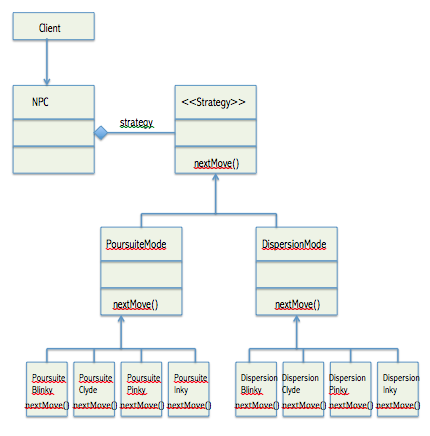
\includegraphics[scale=0.9]{ressources/StrategyDP.png}
		\caption{Design pattern strategy appliqué}
\end{figure}
\newpage

Les quatre classes associées au mode poursuite pour chaque fantôme ont été créées. La méthode de poursuite a été copié-collé dans celles-ci. Ces quatre classes héritent de la classe abstraite "PoursuiteMode".
Quatre autres classes ont donc vues le jour, représentant le mode dispersion de chaque fantôme.
Ces quatre classes héritent de la classe abstraite "DispersionMode".
Enfin, "PoursuiteMode" et "DispersionMode" implémente l'interface "Strategy".

Pour la deuxième version du logiciel, l'algorithme de dispersion a été créé.
Afin de pouvoir l'exécuter, des variables d'instance ont été aménagées dans la classe "Ghost". Une variable "atteintHome" de type "String" indique si le fantôme a atteint sa case maison (la case du coin). Un tableau de direction mémorise le chemin qu'il devra emprunter après avoir visité sa case maison. Un autre tableau de direction représente le chemin qu'il doit prendre à la prochaine occurrence et enfin, un "square" représente sa case maison.
Cet algorithme est placé dans la classe "DispersionMode". Les classes filles font appel à cette même méthode.

Dans la troisième version du logiciel, nous avons mis en place la variable "strategy" nous permettant d'alterner entre la dispersion et la poursuite.
De cette manière, une variable de type "String" est placée dans la classe "NPC" qui représente la stratégie en cours : "ModeDispersion" ou "ModePoursuite". Lorsque la stratégie change au cours du temps, cette variable est modifiée grâce à "setStrategy".
Par exemple, la méthode "nextMove()" de Blinky appelle directement la méthode de sa classe de dispersion ou de sa classe de poursuite associées en fonction de la valeur de cette variable.
Par conséquent, si l'on souhaite modifier la stratégie d'un fantôme, nous n'avons plus à changer le code dans toutes les classes fantômes mais à rectifier les appels aux méthodes.

Enfin, pour la quatrième et dernière version du logiciel, nous avons indiqué au programme de permuter entre les deux stratégies en fonction du temps.
Dans la classe "NpcMoveTask", une variable "temps" est créé pour suivre l'écoulement du temps. Celle-ci est incrémentée à chaque occurrence de la fonction "run" selon la moyenne d'intervalle entre deux coups d'un fantôme. 
Dans la fonction "run", suivant la valeur de cette variable, nous appelons la méthode "setStrategy" de la classe "NPC" afin de modifier la stratégie des fantômes.

\section{Difficultés liées à la fusion}
Concernat la fusion entre la fonctionnalité "Supergomme" et la fonctionnalité "Série de labyrinthe", nous n'avons eu aucun conflit et le jeu était en parfait état de marche lorsque les deux fonctionnalités s'exécutaient en même temps.

Concernant la fusion avec la troisième fonctionnalité, quelques conflits se sont présentés, notamment dans les classes "MapParser" ainsi que dans les classes des fantômes (Blinky, Clyde, Inky et Pinky) néanmois cela s'est assez vite réglé car nos codes étaient tout de même compatibles.

Pour lancer la version finale contenant les trois fonctionnalités, il suffit de démarrer la classe "LaunchSuperPellet".

\section{Analyse de la qualité du code}
\subsection{Outils utilisés}
\subsubsection{Google CodePro AnalitiX}
Le premier outil utilisé est Google CodePro AnalitiX sous sa forme
plugin Eclipse.

Il s'agit d'un outil très complet qui permet le calcul des métriques,
la détection de code dupliqué, l'analyse des dépendances et la couverture
du code et des tests. Dans cette situation, nous l'utilisons pour le calcul des métriques,
la détection de code dupliqué et l'analyse des dépendances.

\subsubsection{EclEmma}
Le second outil est Emma sous sa forme plugin Eclipse (EclEmma).

Emma est un outil utilisé pour vérifier la couverture du code ainsi
que les tests lors de l'exécution de ces derniers.

\subsubsection{CodeCity}
Le troisième outil est CodeCity.

CodeCity est un outil qui permet de visualiser les métriques sous
forme graphique. Nous l'avons utilisé pour constater les différences
entre le projet de base et le projet modifié.

\subsubsection{PMD}
Le dernier outil utilisé est PMD sous sa forme plugin Eclipse.

PMD est un logiciel permettant de détecter les mauvaises pratiques
de programmation ("Bad Smells"). Nous avons observé la variation
de l'apparition de ces "Bad Smells" lors de la modification du
projet.

\subsection{Analyse des dépendances}
\subsubsection{Projet de base}
La Figure 1 est un graphe des dépendances entre les packages
du projet de base. Il est possible de constaté sur celui-ci beaucoup de
dépendances cycliques ainsi que certaines classes ayant une forte interdépendance (exemple: "ghost" et "level").

\begin{figure}[!h]
\begin{center}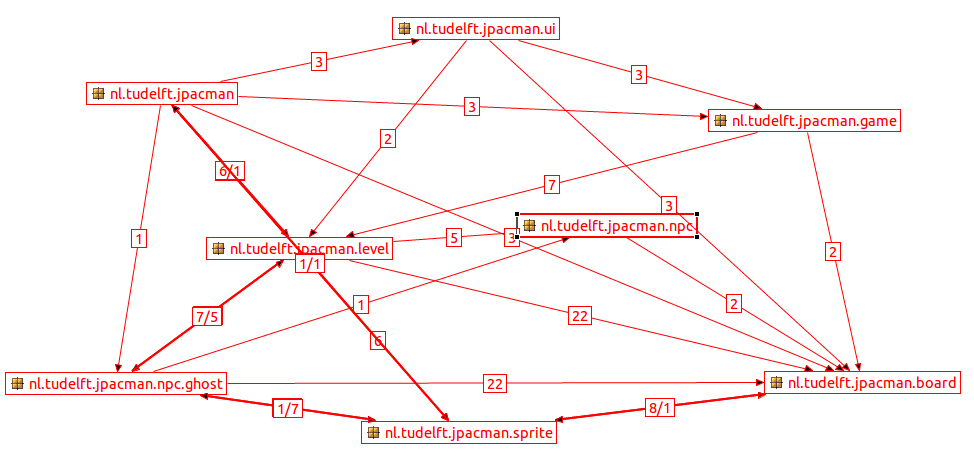
\includegraphics[scale=0.5]{ressources/final_initial_dependencies}\end{center}
\caption{Dépendances du projet de base}
\end{figure}

\subsubsection{Projet modifié}
Un graphe des dépendances est représenté à la Figure 2. Celle-ci permet de constater qu'en général les dépendances ont augmenté et que nous avons aussi
ajouté des interdépendance entre deux packages qui n'en possédaient
pas.

\begin{figure}[!h]
\begin{center}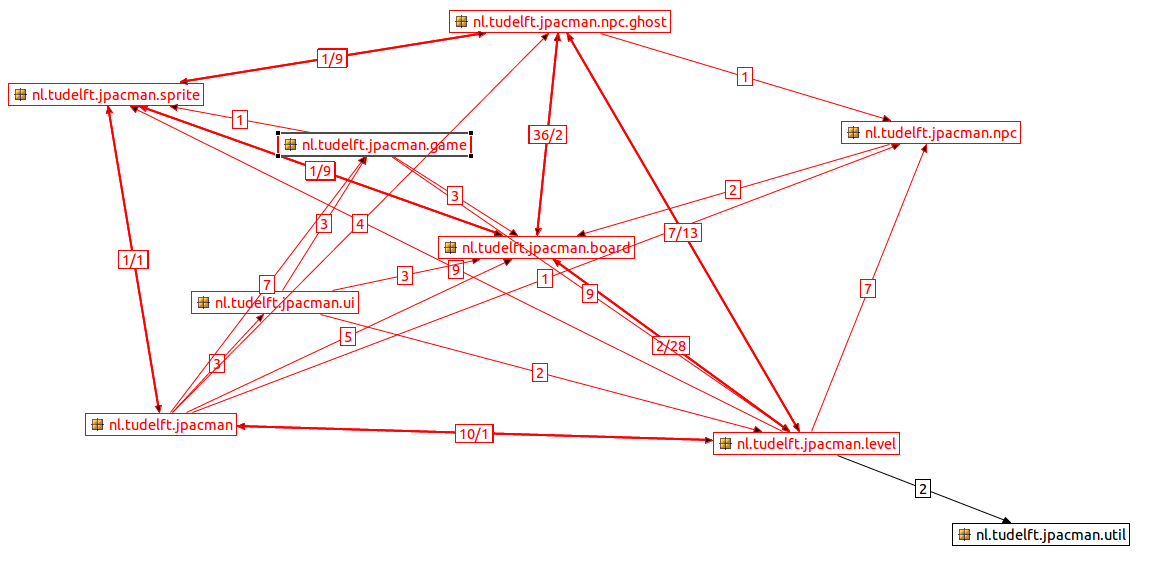
\includegraphics[scale=0.5]{ressources/final_new_dependencies}\end{center}\caption{Dépendances du projet modifié}


\end{figure}

\subsection{Code dupliqué}
Selon Google CodePro AnalitiX, il y a 54 lignes de code dupliquées
dans le projet de base. Cette valeur est assez basse et démontre la
volonté des développeurs du projet d'éviter la programmation "copiée-collée"

Suite à nos modification, Google CodePro AnalitiX, pointe toujours 54 lignes de code dupliquées,
nous n'avons donc pas altéré ce point précis du code lors de nos modifications.


\subsection{Test \& Code Coverage}
\subsubsection{Projet de base}
EclEmma nous donne comme valeurs:
\begin{itemize}
\item Test coverage : 80.9\%.
\item Code coverage (exécution sans jouer) : 41\%.
\item Code coverage (exécution partie type): $\sim$60\%.
\end{itemize}

\subsubsection{Projet modifié}
EclEmma nous donne comme valeurs:
\begin{itemize}
\item Test coverage : 71\%.
\item Code coverage (exécution sans jouer) : 35.9\%.
\item Code coverage (exécution partie type): $\sim$60\%.
\end{itemize}
Nous constatons que de manière générale le coverage a diminué, principalement
au niveau du test coverage. Bien qu'un paradigme de programmation
défensive a été utilisé, nous n'avons pas réussi à trouver de tests
qui couvrent l'entièreté du code ajouté.

\subsection{Métriques}
\subsubsection{Tableaux de métriques}
La Figure 3 présente les deux tableaux de métriques parallèlement l'un à l'autre, ce
qui permet de comparer facilement les résultats.

Il est possible de noter, entre autres, une légère augmentation de la complexité
cyclomatique, un accroissement général de la taille des différentes
classes (nombre de méthodes et nombre de lignes) et une légère diminution
du ratio des commentaires.

\begin{figure}[!h]
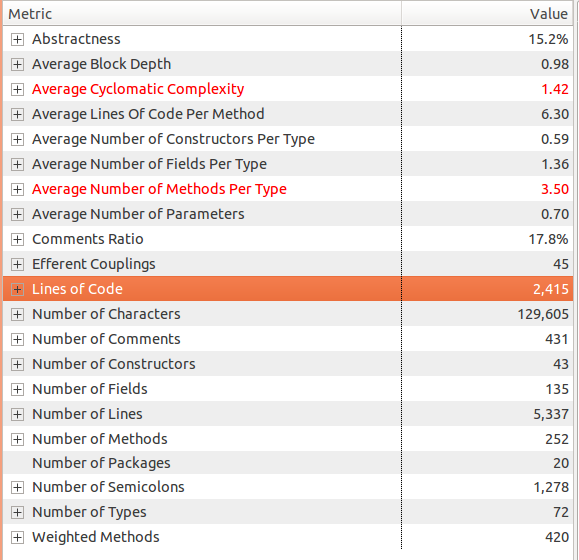
\includegraphics[scale=0.45]{ressources/final_initial_metrics}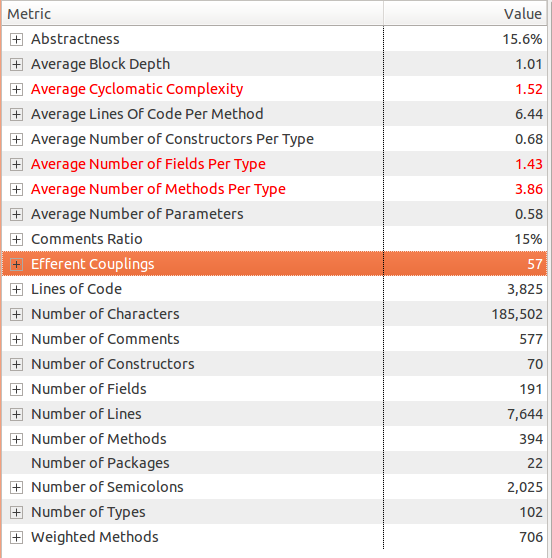
\includegraphics[scale=0.45]{ressources/final_new_metrics}\caption{Comparaison des tableaux de métriques (initial à gauche)}


\end{figure}

\subsubsection{CodeCity : méthodes par classes}
Codecity nous a permis de représenter graphiquement certaines métriques
par classes sur l'ensemble du projet.

Dans ce cas, nous nous intéressons au nombre de méthodes par classe. Nous constatons que de manière générale, celui augmente pour l'ensemble du projet.

\begin{figure}[!h]
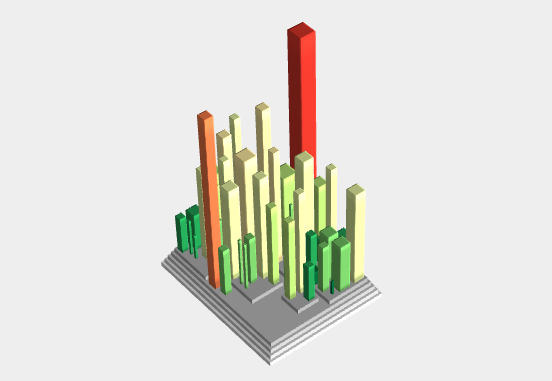
\includegraphics[scale=0.5]{ressources/final_initial_declared_methods}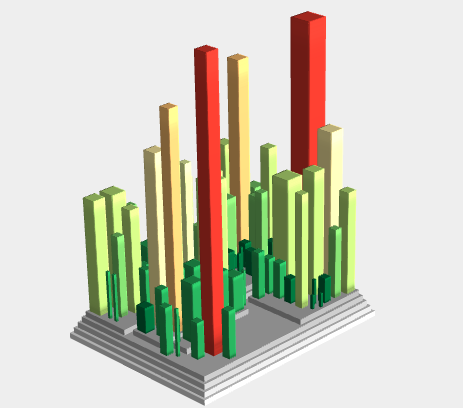
\includegraphics[scale=0.5]{ressources/final_new_declared_methods}\caption{Comparaison du nombre de méthodes par classe (initial à gauche)}


\end{figure}

\subsubsection{CodeCity : complexité cyclomatique}
La Figure 5 démontre que la complexité cyclomatique reste sensiblement
la même.

\begin{figure}[!h]
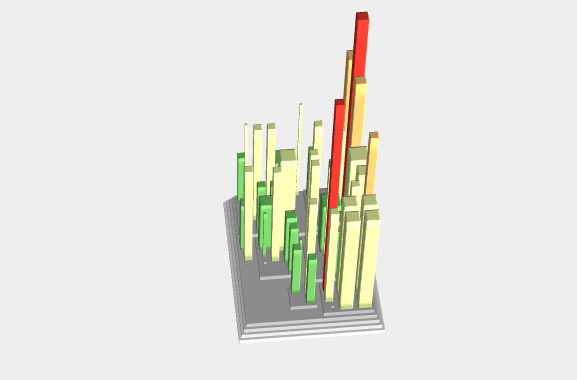
\includegraphics[scale=0.5]{ressources/final_initial_cyclomatic}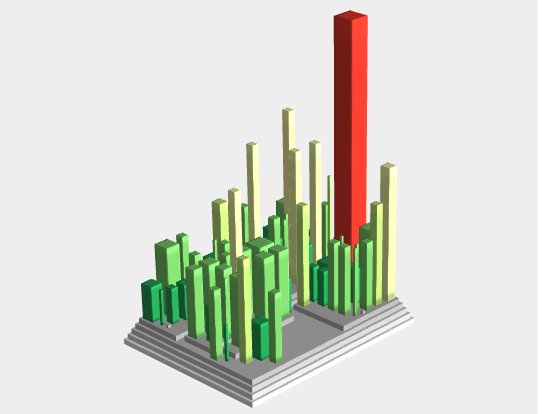
\includegraphics[scale=0.5]{ressources/final_new_cyclomatic}\caption{Comparaison de la complexité cyclomatique par classe (initial à gauche)}


\end{figure}

\subsubsection{CodeCity : nombre de lignes de code}
Sur la Figure 6, le nombre de lignes de code par
classe est resté sensiblement identique, excepté pour deux d'entre elles
("Launcher" et "Level") qui mériteraient d'être séparées en plus petites
classes pour éviter le phénomène de "God Class".

\begin{figure}[!h]
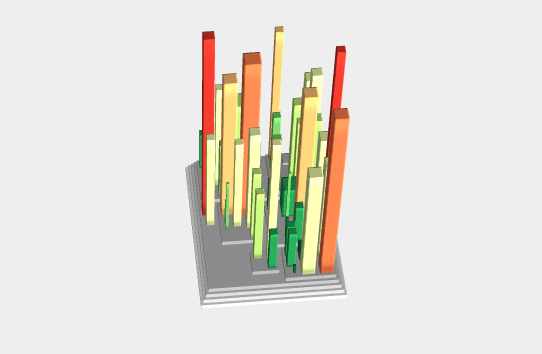
\includegraphics[scale=0.5]{ressources/final_initial_lines_of_code}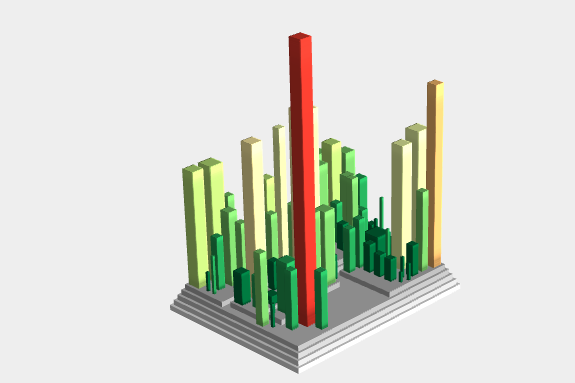
\includegraphics[scale=0.5]{ressources/final_new_lines_of_code}\caption{Comparaison du nombre de lignes de code par classe (initial à gauche)}


\end{figure}

\subsection{Bad Smells}
PMD a mis en évidence 827 violations des bonnes pratiques de programmation
dans le projet initial. En ce qui concerne le projet final, les violation montent à 1442. Les erreurs les plus fréquentes sont "variable
or argument could be final" (39.6\% des violations pour le projet
initial contre 33\% pour le projet modifié), "law of demeter"
(10\% pour le projet initial contre 12\% pour le projet modifié) et
"short variable" (10\% pour le projet initial contre 11\% pour
le projet modifié).

Nous avons donc un accroisement de 74\% de violations selon PMD, à savoir
que le code est passé de 2415 à 3825 lignes de code, c'est à dire
un accroissement de 58\% en ce qui concerne la taille du projet en terme de nombre
lignes de codes (lignes de code effectives selon Google CodePro AnalitiX).
Notons également que PMD nous donne deux avertissements pour "God Class"
concernant les classes "Level" et "Launcher". Ces deux classes ont subi une grande croissance lors nos
modifications respectives. Il semble qu'un refactoring soit nécessaire
à ce niveau pour pouvoir poursuivre la maintenance logicielle.

\section{Conclusion}
\end{document}